%%
%% Copyright 2007, 2008, 2009 Elsevier Ltd
%%
%% This file is part of the 'Elsarticle Bundle'.
%% ---------------------------------------------
%%
%% It may be distributed under the conditions of the LaTeX Project Public
%% License, either version 1.2 of this license or (at your option) any
%% later version.  The latest version of this license is in
%%    http://www.latex-project.org/lppl.txt
%% and version 1.2 or later is part of all distributions of LaTeX
%% version 1999/12/01 or later.
%%
%% The list of all files belonging to the 'Elsarticle Bundle' is
%% given in the file `manifest.txt'.
%%

%% Template article for Elsevier's document class `elsarticle'
%% with numbered style bibliographic references
%% SP 2008/03/01
%%
%%
%%
%% $Id: elsarticle-template-num.tex 4 2009-10-24 08:22:58Z rishi $
%%
%%

%\documentclass[preprint,12pt]{elsarticle}

%% Use the option review to obtain double line spacing
%%\documentclass[preprint,review,12pt]{elsarticle}

%% Use the options 1p,twocolumn; 3p; 3p,twocolumn; 5p; or 5p,twocolumn
%% for a journal layout:
%% \documentclass[final,1p,times]{elsarticle}
%% \documentclass[final,1p,times,twocolumn]{elsarticle}
%% \documentclass[final,3p,times]{elsarticle}
%% \documentclass[final,3p,times,twocolumn]{elsarticle}
%% \documentclass[final,5p,times]{elsarticle}
\documentclass[final,5p,times,twocolumn]{elsarticle}

%% if you use PostScript figures in your article
%% use the graphics package for simple commands
%% \usepackage{graphics}
%% or use the graphicx package for more complicated commands
\usepackage{graphicx}
%% or use the epsfig package if you prefer to use the old commands
%% \usepackage{epsfig}

%% The amssymb package provides various useful mathematical symbols
\usepackage{amssymb}
%% The amsthm package provides extended theorem environments
%% \usepackage{amsthm}

%% The lineno packages adds line numbers. Start line numbering with
%% \begin{linenumbers}, end it with \end{linenumbers}. Or switch it on
%% for the whole article with \linenumbers after \end{frontmatter}.
%% \usepackage{lineno}

%% natbib.sty is loaded by default. However, natbib options can be
%% provided with \biboptions{...} command. Following options are
%% valid:

%%   round  -  round parentheses are used (default)
%%   square -  square brackets are used   [option]
%%   curly  -  curly braces are used      {option}
%%   angle  -  angle brackets are used    <option>
%%   semicolon  -  multiple citations separated by semi-colon
%%   colon  - same as semicolon, an earlier confusion
%%   comma  -  separated by comma
%%   numbers-  selects numerical citations
%%   super  -  numerical citations as superscripts
%%   sort   -  sorts multiple citations according to order in ref. list
%%   sort&compress   -  like sort, but also compresses numerical citations
%%   compress - compresses without sorting
%%
%% \biboptions{comma,round}

% \biboptions{}


\journal{Journal of Chromatography B}

\usepackage{color}
\newcommand\red[1]{{\color{red}#1}}

\begin{document}

\begin{frontmatter}

%% Title, authors and addresses

%% use the tnoteref command within \title for footnotes;
%% use the tnotetext command for the associated footnote;
%% use the fnref command within \author or \address for footnotes;
%% use the fntext command for the associated footnote;
%% use the corref command within \author for corresponding author footnotes;
%% use the cortext command for the associated footnote;
%% use the ead command for the email address,
%% and the form \ead[url] for the home page:
%%
%% \title{Title\tnoteref{label1}}
%% \tnotetext[label1]{}
%% \author{Name\corref{cor1}\fnref{label2}}
%% \ead{email address}
%% \ead[url]{home page}
%% \fntext[label2]{}
%% \cortext[cor1]{}
%% \address{Address\fnref{label3}}
%% \fntext[label3]{}

%& SHORT COMMUNICATION about 2850 words 
\title{Integrated enrichment analysis and pathway-centered visualization of metabolomics, proteomics, transcriptomics, and genomics data by using the InCroMAP software}

%% use optional labels to link authors explicitly to addresses:
%% \author[label1,label2]{<author name>}
%% \address[label1]{<address>}
%% \address[label2]{<address>}

\author[uni]{Johannes Eichner\fnref{eqc}}
\author[uni]{Lars Rosenbaum\corref{cor}\fnref{eqc}}
\ead{lars.rosenbaum@uni-tuebingen.de}
\author[uni]{Clemens Wrzodek}
\author[idm,endo,dzd]{Hans-Ulrich H\"aring}
\author[uni]{Andreas Zell}
\author[idm,zentrallabor,dzd]{Rainer Lehmann\corref{cor}}
\ead{rainer.lehmann@med.uni-tuebingen.de}
\address[uni]{Center for Bioinformatics, University of T\"ubingen, T\"ubingen, Germany}
\address[idm]{Institute for Diabetes Research and Metabolic Diseases of the Helmholtz Centre Munich at the University of T\"ubingen, T\"ubingen, Germany}
\address[endo]{Division of Endocrinology, Diabetology, Vascular Medicine, Nephrology and Clinical Chemistry, Department of Internal Medicine IV, University Hospital T\"ubingen, T\"ubingen, Germany}
\address[zentrallabor]{Division of Clinical Chemistry and Pathobiochemistry, Department of Internal Medicine IV, University Hospital T\"ubingen, T\"ubingen, Germany}
\address[dzd]{German Center for Diabetes Research (DZD), Germany}

\cortext[cor]{Corresponding authors. Tel. +49-7071-29-8 31 93}
\fntext[eqc]{These two authors contributed equally to this work.}

\begin{abstract}
%% Text of abstract
In systems biology, the combination of multiple types of omics data, such as metabolomics, proteomics, transcriptomics, and genomics, yields more information on a biological process than the analysis of a single type of data. Thus, data from different omics platforms is usually combined in one experimental setup to obtain insight into a biological process or a disease state. Particularly high accuracy metabolomics data from modern mass spectrometry instruments is currently more and more integrated into biological studies. Reflecting this trend, we extended InCroMAP, a data integration, analysis and visualization tool for genomics, transcriptomics, and proteomics data. Now, the tool is able to perform an integrated enrichment analysis and pathway-based visualization of multi-omics data and thus, it is suitable for the evaluation of comprehensive systems biology studies.
\end{abstract}

\begin{keyword}
%% keywords here, in the form: keyword \sep keyword
Metabolomics \sep Transcriptomics \sep Proteomics \sep Genomics \sep Systems biology \sep Enrichment analysis \sep Pathway visualization \sep Bioinformatics
%% MSC codes here, in the form: \MSC code \sep code
%% or \MSC[2008] code \sep code (2000 is the default)

\end{keyword}

\end{frontmatter}

%%
%% Start line numbering here if you want
%%
% \linenumbers

%% main text
\section{Introduction}
Today, high-throughput methods for the analysis of biological systems, such as microarrays, next generation sequencing, as well as mass spectrometric and NMR approaches generate a wealth of omics-scale data. To develop hypotheses about a biological process or a disease state, a variety of omics platforms for measuring different genomic, proteomic, and metabolomic features are combined in one experimental setup. Probably the most frequently analyzed genomic feature is messenger RNA (mRNA), which can be quantified on a genome-wide level by gene expression chips (microarrays) or next generation sequencing techniques. Other important (epi)genomic features include microRNA (miRNA), single-nucleotide polymorphisms (SNPs), and epigenetic information, such as the promoter methylation status (DNAm). Proteomic features can be derived from abundance profiling of particular protein patterns and posttranslational modifications, such as acetylation and phosphorylation. Furthermore, mass spectrometric and NMR-based 
metabolomics platforms allow to investigate complex metabolite patterns with high accuracy. In recent years, increasing attention has been drawn to the integration of metabolomics with molecular profiling on the transcriptional and protein level \cite{Gruden2012, Amiour2012}.
The sensible and integrated visualization of omics data at different levels of abstraction is crucial to obtain biological insight without being overwhelmed by the intrinsic complexity of the data \cite{Gehlenborg2010}. A key concept for detecting alterations in cell signalling or metabolism in a biological system are pathway-based visualizations.

A plethora of tools were developed for the inspection of data from individual platforms (see \cite{Gehlenborg2010} for examples). Furthermore, solutions for the combined visualization of transcriptomics (mRNA) and metabolomics data exist \cite{Garcia-Alcalde2011,Waegele2012}. Both Paintomics \cite{Garcia-Alcalde2011} and MassTRIX \cite{Waegele2012} are web-service based tools that are capable of visualizing mRNA microarray and identified metabolomics data in KEGG pathways \cite{Kanehisa2012}. MassTRIX is able to handle unidentified metabolic data by comparing each mass against theoretical adducts stored in metabolomics databases. An example of a tool that can handle several heterogeneous types of omics data is the commercial Ingenuity Pathway Analysis software (www.ingenuity.com). However, Ingenuity does not provide an integrated visualization of multi-level omics data. In summary, the comprehensive analysis of multi-omics data is presently limited because current high-level analysis tools are not able to 
perform an integrated analysis of data from multiple types of omics platforms, are focused on certain specialized platforms, or not freely available. Thus, novel analysis tools and appropriate visualizations are required, since complex interactions between multiple layers of a biological system can only be inferred by the integration of omics data across multiple platforms.

In this contribution we present an extended version of the tool InCroMAP (Integrated analysis of Cross-platform MicroArray and Pathway data) \cite{Wrzodek2012a,Wrzodek2012b}. InCroMAP is a stand-alone Java software originally developed for the enrichment analysis and pathway-based visualizations of genomic and proteomic data, where multiple biological layers were monitored in the same set of samples. The application was specifically designed to provide a high ease of use for investigators of all kinds of analytical disciplines, i.e. detailed experiences in bioinformatics are not necessary. Consequently, all information required, for example, for the mapping between different metabolite identifiers or the annotation of miRNAs with mRNA targets, is either directly included in the tool or dynamically downloaded in the background. Previous versions of InCroMAP focused on genomics and transcriptomics data and were designed for the combined analysis of a wide variety of omics platform types, where 
each feature can be linked to a gene or genomic interval. Up to the present, metabolomics data was not supported. In the extended version of InCroMAP presented here, we support the enrichment analysis and pathway-based visualization of annotated metabolomics data and thereby complemented the tool for comprehensive systems biology data evaluation. For convenience, InCroMAP supports several commonly used metabolite identifiers, such as specific database identifiers (e.g., HMDB \cite{Wishart2009}), common synonyms, and InChIKeys. 

InCroMAP is freely available under the LGPL3 license at http://www.cogsys.cs.uni-tuebingen.de/software/InCroMAP, including a comprehensive user’s guide and several example data files to test the capabilities of the tool.

\section{Methods}
Before systems biology data from heterogeneous platforms can be integrated and visualized with high-level data analysis tools like InCroMAP, the data has to be preprocessed in a platform-dependent manner (see Figure \ref{fig:incromap-workflow}). A typical workflow for metabolomics data from nontargeted mass spectrometric measurements includes the following steps. First, metabolite features, which are characterized by mass and relative intensity, are extracted from the raw data files by applying software tools, like our recently developed FeatureFinder software \cite{Kenar2014} or commercial tools implemented in the software of the instrument. Ideally, the feature induced by a metabolite should contain all signals that were generated by the metabolite (including isotopic peaks) \cite{Kenar2014}. Second, the extracted features have to be aligned and linked between the different samples. The aforementioned preprocessing steps can be performed with sophisticated open-source software tools like OpenMS \cite{
Sturm2008}. The features are then subjected to quality controls and low-level statistical data analysis, which includes normalization and calculation of measures for differential abundance between conditions (e.g., p-values, fold changes, or log ratios). Mostly, these tasks are performed with commercial statistics software, open-source omics analysis applications like Mayday \cite{Battke2010}, or directly with the statistical programming language R (www.r-project.org). In a final preprocessing step, the metabolite features are annotated with candidate identifiers using information provided by metabolomics databases, such as PubChem \cite{Wang2009}, HMDB \cite{Wishart2009}, or LIPID MAPS \cite{Sud2007}. Similar preprocessing workflows exist for other platforms, like microarrays, next generation sequencing, and proteomics. The processed data can then be imported and analyzed with InCroMAP.

In a typical use case of InCroMAP (see Figure \ref{fig:incromap-workflow}), the user first imports his preprocessed multi-level omics data, given in tabular format. Then, the differing metabolites, genes and proteins are determined for each platform, based on appropriate cutoffs. Next, relevant pathways related to the biological background of the experiments are inferred. For the detection of relevant pathways, InCroMAP employs a special pathway enrichment algorithm, which integrates differing metabolites, genes, and proteins across multiple platforms. The resulting pathways can then be selected for further visual inspection from a table in which each pathway is associated with a significance value. Alternatively, the metabolic overview function of InCroMAP can be used to generate an interactive global map of cellular metabolism, in which each subordinate metabolic pathway is colored according to the significance of its enrichment. The results of the enrichment analysis can be 
exported in tabular format and the pathway-based visualizations can be easily stored as JPEG images.

\begin{figure*}
\center
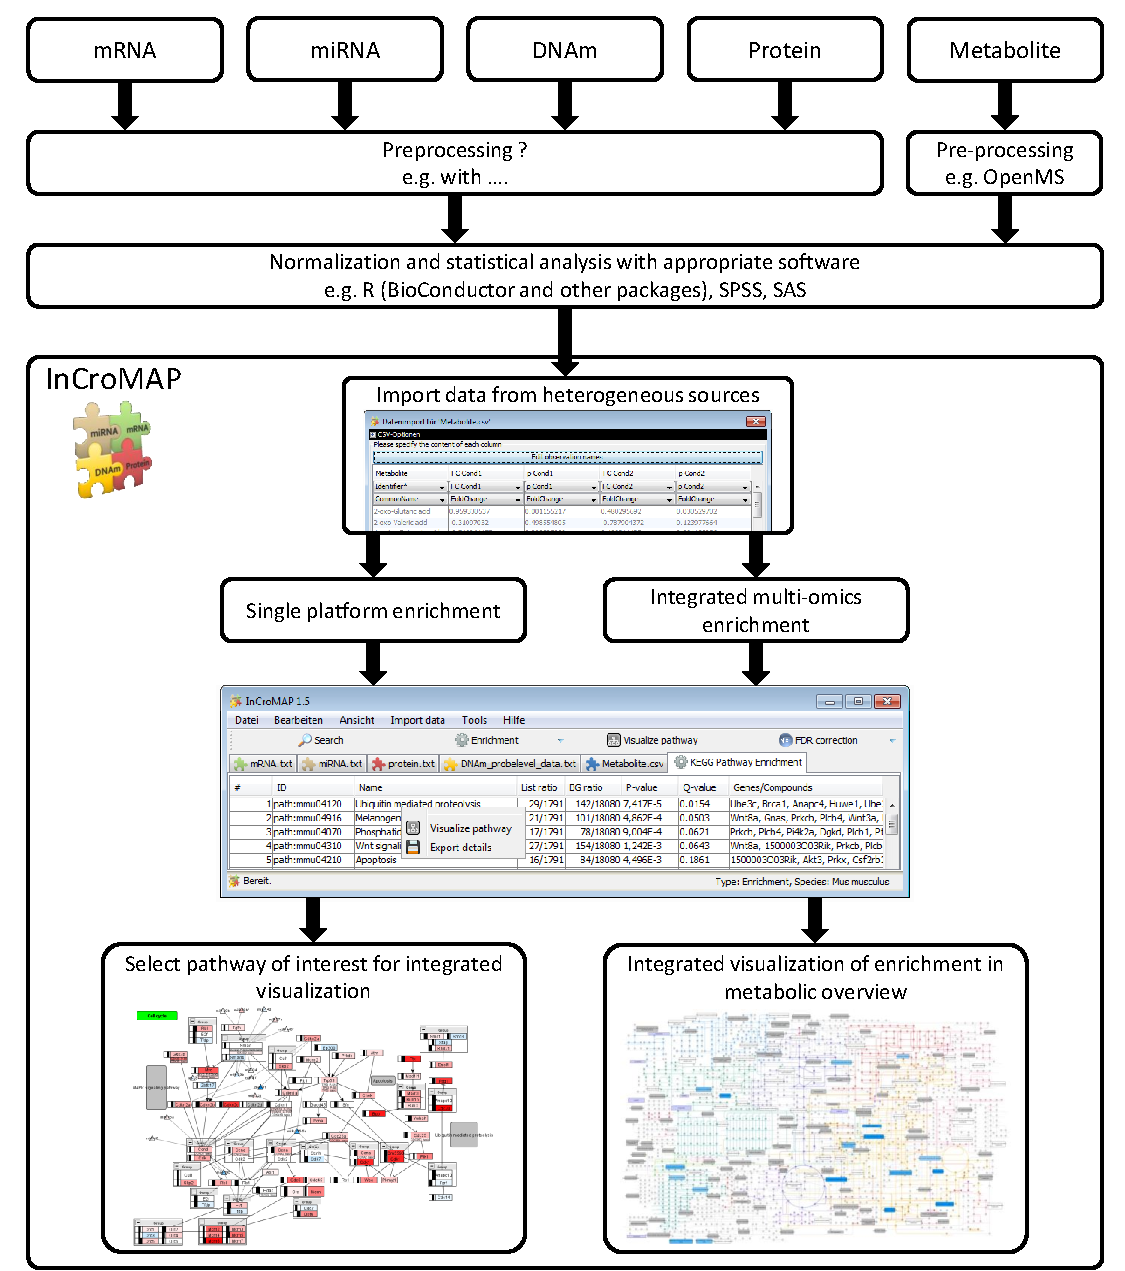
\includegraphics[width=0.85\textwidth]{InCroMAP_workflow.pdf}
\caption{The flow chart depicts the general workflow of an analysis with InCroMAP. The raw data from each platform is preprocessed using appropriate, platform-specific algorithms for data preparation (e.g., feature extraction) and the alleviation of experimental artifacts (e.g., normalization techniques). Then, the data is analyzed with a statistics software, which yields p-values or fold changes for each of the features. Finally, the gene, protein, and metabolite features are annotated with candidate identifiers. After these preprocessing steps the data can be easily imported to InCroMAP and an enrichment analysis can be performed. On the basis of the enrichment, the user may select a pathway of interest, which can be overlaid with the corresponding omics data. Alternatively, a visualization showing a global metabolic overview of the alterations in pathways can be generated.}
\label{fig:incromap-workflow}
\end{figure*}

\subsection{Data import}
InCroMAP software uses an intuitive, largely uniform input format for the import of heterogeneous types of processed omics data. The software accepts tabular input files (e.g., CSV files exported from MS Excel) which consist of platform-dependent metadata columns containing appropriate identifiers (e.g., Affymetrix, EntrezGene, HMDB IDs, etc.) and data columns corresponding to the fold-changes or p-values calculated for a particular sample group.

InCroMAP is able to handle various types of identifiers for genomics, transcriptomics, proteomics, and metabolomics data. It supports the recognition of identifiers used by the most common oligonucleotide microarray manufacturers (e.g., Affymetrix, Agilent, etc.). Additionally, generic formats facilitate the import of processed data, provided that each measurement can be either associated with a certain gene, genomic region, protein, or metabolite. For miRNA data the systematic name (i.e., miRBase ID) has to be provided. The miRNA transcripts can then be automatically connected to canonical pathways based on confirmed or predicted interactions with potential target mRNAs. Protein data is simply linked to the corresponding genes. Since diverse proteins corresponding to the same gene may have been measured, a gene identifier as well as an arbitrary identifier for the protein modification has to be provided. Metabolomics data may be annotated by a database identifier (e.g., KEGG, HMDB, PubChem, LIPID MAPS), an InChIKey, or a common synonym. Internally, all metabolites are mapped to InChIKeys. Pathways of interest can either be automatically downloaded from KEGG or imported from other sources (e.g., Reactome, BioCarta, etc.) in BioPAX format \cite{Eustachio2011}.

We decided to use InChiKeys as internal identifier for metabolites because they are a compact, almost certainly unique identifier, which does not change as frequently as most database identifiers. We merged the dumps of four different compound databases (HMDB, LIPIDMAPS, KEGG, and PubChem) based on the InChIKeys with self-made python scripts and kept only entries with information for at least two different databases. Entries without InChIKey information, e.g. information on compound classes,  were discarded. In principal, the information can be mapped on actual compounds using taxonomies, but this procedure might introduce errors in the generated mapping database.

\subsection{Enrichment analysis}
The InCroMAP software allows for the calculation of single-platform and cross-platform enrichments, based on omics experiments from individual and multiple platforms, respectively. In the former case, a hypergeometric test is applied to assess the significance of the overrepresentation of predefined gene sets (e.g., KEGG pathways) within a list of differing genes derived from a certain experiment based on fold-change and/or p-value cutoffs. The same statistical approach is used to determine pathways enriched with differing metabolites. In both cases, the union of all genes/metabolites in KEGG is considered as the universe. For the calculation of metabolite set enrichments a variety of other tools (e.g., MSEA, MBRole, MPEA, etc.) have been developed \cite{Xia2010,Chagoyen2011,Kankainen2011}, some of which also include implementations of more sophisticated algorithms accounting for metabolite concentrations. However, these tools do not offer integrated enrichment analysis across multiple platforms. For this purpose, InCroMAP uses a straightforward extension of the single-platform method. Specifically, a hypergeometric test is used, where the sample corresponds to the union of the molecules which were changed in terms of abundance on any of the platforms and the universe is given by the union of the platform-specific background sets. To our knowledge, the only two alternative methods for calculating an integrated enrichment based on both transcriptomics and metabolomics data are implemented in the tools IMPaLA \cite{Kamburov2011} and Paintomics \cite{Garcia-Alcalde2011}. Paintomics also calculates the integrated enrichment p-values based on a hypergeometric test, but the details remain unclear from the publication. In contrast to our software, IMPaLA calculates the enrichment p-values independently for each platform using either a hypergeometric test or Wilcoxon enrichment analysis. As the experiments are considered independent, the joint p-value is then computed based on the product of the p-values calculated for the individual platforms. Like IMPaLA, InCroMAP supports a wide variety of source databases, such as KEGG pathways (including proteins/compounds), gene sets from the molecular signatures database (MSigDB), and gene ontology (GO) terms. The result list of an exemplary KEGG pathway enrichment is depicted in Figure \ref{fig:incromap-workflow}, where each pathway is assigned a p-value and an FDR corrected p-value (q-value).

During the enrichment analysis, InCroMAP discards unidientified features that could not be mapped to a gene or metabolite. While this procedure results in a loss of information, there is currently no better way to handle the problem of unidentified features. Generally, InCroMAP is not limited to targeted metabolomics data because dedicated tools, such as OpenMS or XCMS, are able to assign multiple candidate identifiers to metabolic features. However, the annotation with multiple candidate identifiers usually yields many-to-many mappings because a metabolic feature can be mapped to several candidate identifiers and vice versa. These many-to-many mappings are problematic for the overrepresentation analysis. A user should be careful when interpreting enrichment p-values of untargeted metabolomics data. Solutions to this problem in the setting of gene set enrichment have been proposed \cite{Kankainen2011} and will be evaluated for implementation in a future version of InCroMAP.

\begin{figure*}
\center
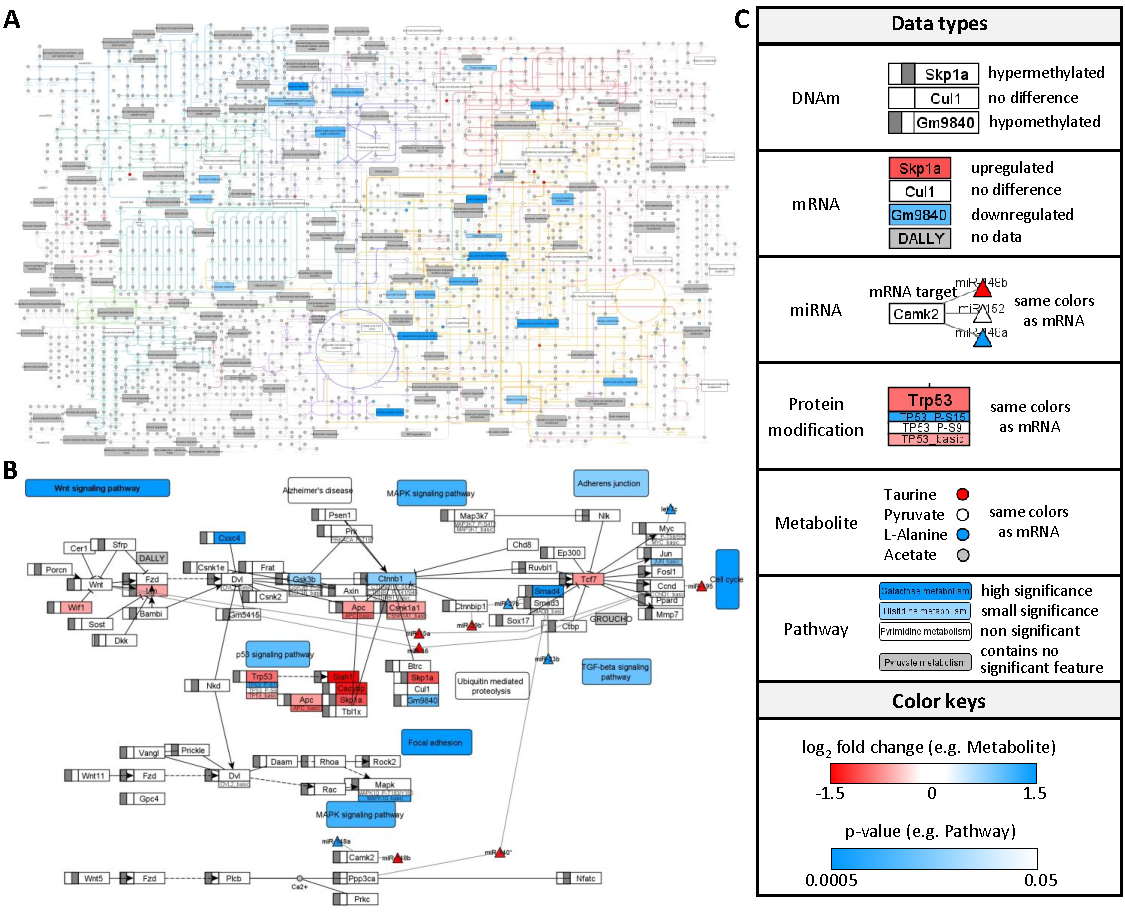
\includegraphics[width=0.85\textwidth]{InCroMAP_examples.pdf}
\caption{\red{The evaluation and visualization of complex multi–omics data in the context of metabolic pathways affected in CTNNB1-mutated mouse liver tumors by the application of InCroMAP is exemplarily shown. (A) shows the metabolic overview in which subordinate metabolic pathways are colored according to their enrichment p-values. Additionally, changes
in concentration are indicated for specific metabolites (highlighted in yellow) which could be identified based on NMR spectroscopy. (B) depicts an excerpt from the Glycolysis / Gluconeogenesis pathway overlaid with omics data obtained from diverse molecular levels (e.g., mRNA/miRNA expression, DNA methylation status of promoters, metabolite concentrations determined by NMR analysis). (C) Taurine and hypotaurine metabolism pathway overlaid with multi-level omics data; D) shows a legend that explains the visualization of the data types and the coloring schemes.}}
\label{fig:incromap-examples}
\end{figure*}

\begin{table*}
\center
\caption{Comparison between chosen features of four different freely available tools for the analysis of multi-omics data. Supported features are marked by a bullet ($\bullet$), whereas non-supported features are indicated by a circle ($\circ$).}
\begin{tabular}{ccccc}
\hline
 & InCroMAP & Paintomics & MassTRIX & IMPaLA\\
\hline
Mass annotation & $\circ$ & $\circ$ & $\bullet$ & $\circ$ \\
Supporting probe-level data & $\bullet$  & $\bullet$  & $\bullet$  & $\circ$ \\
Integrated enrichment analysis & $\bullet$  & $\bullet$ & $\circ$  & $\bullet$  \\
Visualization of pathways & $\bullet$ & $\bullet$ & $\bullet$  & $\circ$\\
Gradual coloring & $\bullet$  & $\bullet$ & $\circ$ & $\circ$\\
Interactive analysis & $\bullet$  & $\circ$ & $\circ$ & $\circ$\\
Metabolic overview  & $\bullet$  & $\circ$ & $\circ$ & $\circ$\\
Analysis of more than two data types & $\bullet$  & $\circ$ & $\circ$ & $\circ$ \\
\hline
\end{tabular}
\label{tab:incromap-comparison}
\end{table*}

\section{\red{Results and discussion}}

\subsection{Metabolic overview}
The results of a pathway enrichment analysis are typically presented to the user as a table or barplot of pathways, sorted according to the associated p-values, which score the significance of the enrichment with differing genes. As these traditional presentations of an enrichment result do not highlight any functional relations between pathways we devised an alternative method, which provides the user with a more structured view of the metabolic pathways altered by a certain condition. Using the metabolic overview feature, the user can display enrichment results in the context of KEGG's global `Metabolic Pathways' map (KEGG: map01100), which contains references to all subordinate metabolic KEGG pathways. In this illustration, pathways, which are significantly enriched with up- or down-regulated genes or metabolites, are highlighted in different shades of blue (Figure \ref{fig:incromap-examples}). Since KEGG does not offer a meta-pathway for cellular signal transduction, this feature is limited to metabolic 
pathways. 

In a recent study, we employed InCroMAP to detect changes in the intermediary metabolism of mouse liver tumors caused by mutations in the oncoproteins CTNNB1 and Ras which play a central role in the Wnt and MAPK signaling pathway, respectively \cite{Unterberger2014}. \red{In order to exemplify the utility of the metabolic overview feature demonstrated in Figure \ref{fig:incromap-examples}A, we applied InCroMAP to multi-level omics data, which are available from GEO under accession GSE51358. Besides metabolite levels detected by NMR this dataset comprises mRNA, miRNA and protein expression as well as DNA methylation profiles.}

\subsection{Pathway-based visualization}
Metabolic or signaling pathways of interest can either be automatically downloaded from KEGG or imported from other sources in BioPAX format. Being rendered in an interactive graph viewer, the pathway nodes representing genes/proteins can be overlaid with expression data from mRNAs and multiple protein products (Figure \ref{fig:incromap-examples}B \red{and C}). Additionally, miRNAs can be connected to a given pathway based on experimentally confirmed or predicted interactions to their target mRNAs. If desired, the tool also visualizes differential methylation of proximal gene promoters, which is by default computed based on the largest peak observed in the upstream region of the transcription start site. In the extended version of InCroMAP we also support the visualization of metabolomics data. For each pathway node corresponding to a gene, protein, or metabolite, the individual measurements derived from multiple platforms and/or probesets as well as the DNA methylation profile of the proximal promoter can be inspected in a separate details panel. The integrated visualization of these data in a pathway-centered manner allows for drawing hypotheses and gaining novel biological insights. \red{To illustrate the analytical power of InCroMAP we selected a complex multi-omics dataset including metabolite levels detected by NMR, expression of mRNA, miRNA and proteins as well as DNA methylation profiles which ideally exemplifies the performance of the software tool. These data were achieved by the investigation of a hepatic tumor characterized by a mutation in the oncoprotein CTNNB1. Exemplarily, tumor based effects on glucose catabolic and anabolic pathways (Figure 2B) as well as of taurine and hypotaurine metabolism (Figure 2C) are presented. The InCroMAP evaluation clearly shows tumor associated alterations in DNA methylation, mRNA expression, microRNA as well as metabolite levels. For instance, the two key enzymes G6pc and Pck1 catalyzing rate-limiting steps in glycogenolysis and gluconeogenesis, respectively, were both downregulated in CTNNB1-mutated tumors (G6pc, Fig. 2B). Concurrently, a slight downregulation of glucose levels was observed. Given the integrated view of the pathway one may hypothesize if G6pc expression is silenced by potentially interacting miRNAs or if the the downregulation of Pck1 is caused by the hypermethylation present in the proximal promoter of the gene.} Since this figure only serves for illustrative purposes, the reader is referred to Unterberger \textit{et al.} for a more detailed description of the metabolic alterations found in CTNNB1-mutated mouse liver tumors \cite{Unterberger2014}.
%\red{The second example, based on LC-MS metabolomics and transcriptomics data, shows the results from the investigation of XXXXXXXX (Supplementary Figure 1). Again InCroMAP data evaluation facilitates the illustration as well as the interpretation of data from a complex systems biology approach.}\\

\red{In summary,} we presented an extended version of InCroMAP, which allows the integrated pathway-based visualization of data from multiple omics platforms, such as DNA methylation, mRNA, miRNA, proteins, protein modifications, and metabolomics data. The tool enables a user to interactively browse through and visualize different KEGG pathways. Furthermore, the metabolic overview function of InCroMAP can be used to generate an interactive global map of cellular metabolism, which provides a structured view of the metabolic changes present in a certain experimental condition. The tool provides a useful overview of multi-omics data in the context of metabolic and signalling pathways, which allows a user to gain insight in complex multi-omics data sets. Thus, it facilitates the interpretation of otherwise cumbersome data and enables the generation of initial biological hypotheses.

Table \ref{tab:incromap-comparison} compiles a comparison between InCroMAP and three others tools for the analysis of multi-level omics data: Paintomics, MassTRIX, and IMPaLA. Paintomics is most similar compared to InCroMAP. However, it only visualizes user specified pathways as image, whereas InCroMAP allows for interactively browsing through the pathways. MassTRIX was specifically  designed for metabolomics data and can annotate metabolic features with candidate identifiers, which is not supported by any of the other tools. However, it does not feature an integrated enrichment analysis and does not perform a gradual coloring of the pathways nodes based on the abundance profiles. IMPaLA is an advanced enrichment analysis tool but it does not support probe-level data and does not provide any means of visualization. Furthermore, InCroMAP provides unique features for data analysis and visualization which are not offered by any published software.  Most notably, a structured, global view of the changes in cellular metabolism can be generated by using the metabolic overview feature. Secondly, InCroMAP facilitates the integrated analysis of more than two types of data.

Currently, the pathway enrichment method of InCroMAP is focused on targeted metabolomics data because the overrepresentation analysis is not designed to handle many-to-many mappings, which ususally occur when assigning multiple candidate identifiers to metabolic features. Future versions of InCroMAP must implement a more dedicated enrichment analysis to handle the problem of many-to-many mappings.

Further future improvements concern the integration of visualizations from additional metabolomics and lipidomics databases, such as LIPID MAPS \cite{Sud2007}. Particularly the inclusion of visualizations based on LIPID MAPS pathways can overcome limitations of KEGG with respect to lipidomics data. Additionally, an automatic annotation with candidate identifiers for nontargeted metabolomics data based on the comparison against theoretical adducts of metabolites from metabolomic databases is planned for a future release of InCroMAP. The tool automatically notifies a user if an update is available on the project homepage (http://www.cogsys.cs.uni-tuebingen.de/software/InCroMAP).

To conclude, InCroMAP is a useful tool for the analysis and visualization of complex metabolomics, proteomics, transcriptomics, and genomics data. It is one of the first freely available tools for the interactive visualization of systems biology data, thereby supporting the identification of (pathobiological) alterations in complex multi-omics data sets.

\section{Acknowledgements}
This project was supported by the Competence Network for Diabetes mellitus funded by the BMBF (FkZ 01GI1104A) and a grant from to the German Center for Diabetes Research (DZD eV; 01GI0925). Furthermore, the project received funding from the Innovative Medicine Initiative Joint Undertaking (IMI JU) [115001] (MARCAR project).

%% The Appendices part is started with the command \appendix;
%% appendix sections are then done as normal sections
%% \appendix

%% \section{}
%% \label{}

%% References
%%
%% Following citation commands can be used in the body text:
%% Usage of \cite is as follows:
%%   \cite{key}         ==>>  [#]
%%   \cite[chap. 2]{key} ==>> [#, chap. 2]
%%

%% References with bibTeX database:


\bibliographystyle{elsarticle-num}
\bibliography{literature}

%% Authors are advised to submit their bibtex database files. They are
%% requested to list a bibtex style file in the manuscript if they do
%% not want to use elsarticle-num.bst.

%% References without bibTeX database:

% \begin{thebibliography}{00}

%% \bibitem must have the following form:
%%   \bibitem{key}...
%%

% \bibitem{}

% \end{thebibliography}


\end{document}

%%
%% End of file `elsarticle-template-num.tex'.
